%!TEX root =  proposal.tex



\section{Grounding our work in computational biology applications}
\label{sec:compbio}

%{\color{gray}

In order to give a concrete and application-oriented grounding to our general GPU algorithm and data structure innovations, we have selected computational biology as an initial application area where we will ``prove out'' the library we develop.  We choose this area specifically for three reasons. First, it is data intensive, with the need to process ever growing quantities of sequencing data. Second, the fundamental building blocks often rely on dynamic or irregular computations of the type we hope to enable via the work in this proposal. Finally, given the experience and background of our team, we have the relevant expertise to properly scope target applications in computational biology and to evaluate the relevance of the results we achieve within the context of the existing state-of-the-art solutions within that field.

\paragraph{A computational biology stress test for our GPU data structures.}
Both the volume and variety of genomic sequencing data has been increasing at an ever faster rate, driven by new and improved massively parallel high-throughput sequencing (HTS) technologies.  These technologies are already producing
petabyte-scale datasets~\cite{kodama2012sequence}, and the NIH estimates that ``genomics research will generate between 2 and 40 exabytes of data within the next decade''~\cite{NHGRIDataScience}. Many applications in computational biology (\kmer
analysis~\cite{MarccaisKi11}, single-cell analysis~\cite{he2022alevin}, raw sequence search~\cite{solomon2016fast}, taxonomic classification~\cite{wood2014kraken}, and pangenomics~\cite{computational2018computational})
require processing raw sequencing data at such enormous scales~\cite{kodama2012sequence}. 
%
Often, these applications are bottlenecked by the performance of an underlying core set of data structures, including filters~\cite{PandeyAlBe18, solomon2016fast}, hash tables~\cite{solomon2016fast,almodaresi2022incrementally}, locality sensitive hashing~\cite{Marais2019}, compressed string indexes~\cite{Almodaresi2018Pufferfish}, etc. % \mfc{fill in the rest from the remainder of intro, once we've read it.}. 
Specifically, the scale of the data is such that two main problems arise \textbf{(1)} some analyses are simply not currently feasible with existing data structures and algorithms --- for example, despite the long-standing desire to build a sequence-level index for the entire SRA, existing efforts have not reached this scale~\cite{Karasikov2020, HarrisM20, SolomonK17, almodaresi2022incrementally, AlmodaresiPFJP20,PandeyAlBe18} and \textbf{(2)} other common analyses are feasible, but computationally burdensome, requiring powerful local compute abilities, or leading to increased costs for analyses using cloud compute; this slows down the analysis and discovery cycle, and has led to a scenario in which, in many cases, compute has overtaken data generation as the predominant experiment-related cost~\cite{Muir_2016} (apart from the cost of human labor). 

While GPUs have proven highly-capable in accelerating the analyses that come ``downstream'' of raw data processing, such as nearest neighbor search and dimensionality reduction from single-cell count matrices~\cite{RAPIDS:2022}, much less progress has been made in terms of providing practical solutions for the intensive preprocessing steps that precede such analyses.  To this end, we identify two raw data analysis ``kernels'' that are used broadly throughout sequence bioinformatics. These kernels are bottlenecks in many comp.~bio.~workflows, so making them faster and scaling them to larger data sets will have widespread impact. GPUs offer an avenue to scaling these data structures.  And while GPUs are fast, they are space constrained.  Therefore, we need new data structures and algorithms that are space efficient to speed up these applications.  
%
The kernels are:

\begin{itemize}%[leftmargin=*,nolistsep]
%\begin{itemize}[leftmargin=*,noitemsep,nolistsep]
\item \textbf{\Kmer analysis.}
\Kmer analysis involves representing raw sequencing data as length-$k$ subsequences called \defn{\boldkmers}, and performing analysis on the occurrence, frequency (and sometimes locations) of \kmers in the data sets; the objective is to answer questions about their genomic diversity, abundance variance, taxonomic origins, etc. \Kmer analysis is the first step in numerous computational biology pipelines, e.g., error correction, de Bruijn graph construction, raw sequence search, digital normalization, comparative genomics, genomics assembly, certain approaches to transcript quantification and the taxonomic classification of metagenomic reads, etc.~\cite{wood2014kraken,GeorganasEHG18,hofmeyr2020terabase,solomon2016fast,PatroSailfish:2014,PandeyAlBe18,PandeyBJP17,PandeyBeJo17b}.

Existing tools use both  approximate\footnote{In this proposal, we refer to data structures as \defn{approximate} if they  have only false positives and \defn{lossy} if they can have false negatives.} and exact data structures (e.g., filters vs.\ hash tables) to construct and store \kmer indexes~\cite{MarccaisKi11,PandeyBJP17}.  \Kmer analysis tools such as  Jellyfish~\cite{MarccaisKi11} use a compact filter to identify singleton \kmers and use a hash table to maintain the frequency count and associated metadata (e.g., prefix-suffix extension, read id, etc.) about the \kmers~\cite{hofmeyr2020terabase}. When the metadata is coherent, this can often be exploited to allow much more space-efficient indexing, at least in the static case~\cite{pibiri2022sparse,pibiri2023weighted,fan2023spt,fan2023fulgor}.
As we will see, \kmer analysis is a key part of several of the specific applications we will be addressing. 
%\mab{can somebody (else) name these? Alice, Bob, Eve?}

% \item \textbf{Compressed indexes.}
% FM-index, BWT, comressed suffix array.
\item \textbf{Sequence alignment.} Sequence alignment involves aligning sequences of DNA, RNA, or protein to identify the origin of locus of sequencing reads, or when comparing references to find similar regions that may be a consequence of underlying biological process and to establish evolutionary relationships.
Sequence alignment is used extensively in reference-based analyses, in which sequencing data is aligned against one or more reference genomes, as well as in genomic and metagenomic assembly to map contigs back to the reads during scaffolding. In computational biology applications, sequence alignment is often performed sequence to sequence; among multiple sequences (\emph{multiple sequence alignment}); and between a sequence and a graph where the graph is one of several different variants of a \defn{sequence graph}, representing the genomes of multiple individuals.

Many existing tools use compressed and succinct string indexes such as the BWT~\cite{burrows1994block} and FM-index~\cite{ferragina2000opportunistic}, the r-index~\cite{gagie2018optimal}, compressed suffix arrays~\cite{grossi2000compressed}, and several hashing-based schemes based on \kmers, minimizers, or other types of designed ``seeds''~\cite{li2018minimap2,pibiri2022sparse,sahlin2022strobealign}, as well as dynamic-programming algorithms for sequence alignment.
Compressed and succinct indexes support efficient ``seed'' lookup, which vastly reduces the set of candidate locations where a high-quality alignment might occur, and helps to perform sequence alignment in a memory-efficient manner and enable these tool to scale to large volumes of data.
Some of the most widely used alignment tools across computational biology, such as Bowtie2~\cite{Langmead2012}, BWA-MEM~\cite{li2013aligning}, STAR~\cite{Dobin2012}, perform fast and efficient sequence alignment using such string indexes.
%\mab{Shorten, or just improve writing on bullets}
%Given the large sizes of sequencing datasets, these tools also use hash-based \kmer indexes to seed the sequence alignment to achieve speedups.
\end{itemize}

\noindent
\textbf{These kernels appear time and again as foundational steps in many different types of analyses within computational biology, and rely on a core set of common data structures to achieve performance and scalability.}  We highlight some of these analyses an their relationships to these kernels in~\Cref{fig1}, and describe the specific applications of metagenomic classification and abundance estimation, large-scale sequence search, and pangenomics, that we will use as target applications within this proposal, in~\Cref{subsec:target-applications}. The underlying set of shared data structures that we will build out and apply in this proposal include (i) compact compact and exact data structures: hash tables and succinct bit vectors, compressed string indexes, and trees, as well as (ii) sketches and approximate data structures: filters, cardinality estimators,  min-hash based sketches, and other locality-sensitive hash data structures.

% \setlength\intextsep{0pt}
\begin{wrapfigure}[17]{R}{0.6\textwidth}
% \begin{figure}
\centering
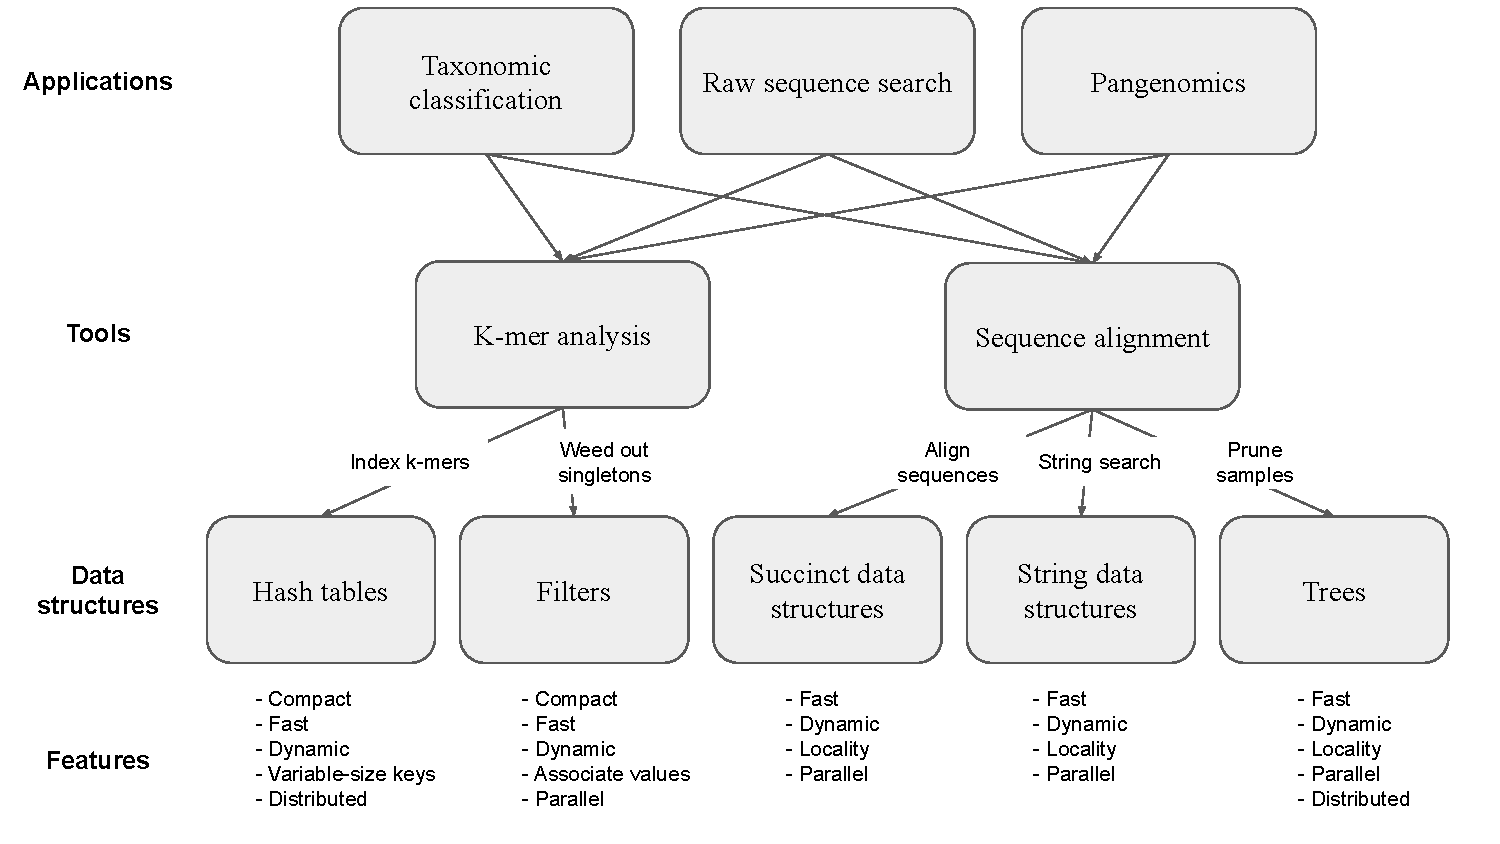
\includegraphics[width=1.0\textwidth]{images/PPOSS_App_DS}
\caption{Relation between computational biology applications, data processing tools and data structures. We further mention the desired features in data structures to achieve performance and scalability.}
\label{fig1}
% \end{figure}
\end{wrapfigure}

The performance and scalability of downstream applications depends on the space-efficiency, speed, dynamism, and scalability of the
underlying data structures they use. In addition to computational biology, these data structures are also the building blocks in many other domains, such as databases, machine learning, software systems, and security applications.

% \mfc{this next paragraph feels redundant.  PRashant, do we just kill it?}

% \paragraph{Existing software tools for computational biology applications.}
% \sout
% {There are numerous tools for \kmer counting~\cite{MarccaisKi11,PandeyBJP17a}, sequence alignment~\cite{altschul1990basic,kielbasa2011adaptive,li2018minimap2,schwartz2003human}, raw sequence search~\cite{solomon2016fast,PandeyABFJP18Cell}, taxonomic classification~\cite{wood2014kraken,wood2019improved}, and pangenomics~\cite{garrison2018variation,pandey2021variantstore}. These tools rely on space-efficient and high-performance CPU data structures such as filters, sketches, hash tables, and string indexes. Most of these tools are designed for shared-memory parallelism and they often do not scale out of shared memory to disks.
% These existing tools are limited by single-node compute and shared-memory parallelism. They are not designed to scale to thousands of cores on modern accelerators nor scale out to hundreds to nodes in a high-performance computing (HPC) environment.
% }
%


\label{sec:we-need-performance-and-scalability}

\begin{comment}
    
\paragraph{CPU speed and RAM capacity cannot keep up with data growth.}
Unfortunately, CPU speed and RAM sizes aren't keeping up with the data growth in computational biology and other applications.
Although CPU performance is increasing at 2--25\%/year and single-node RAM sizes are increasing at 2--11\%/year, genomics data is is likely to double in size every 1.5 years~\cite{kodama2012sequence}.
% See~\Cref{fig:sra_data}.
Thus, today's software tools will not scale with tomorrow's data. For example, performing \kmer analysis or sequence alignment on petabyte-scale raw sequencing data is not possible on single-node shared-memory systems.

In the post-Moore’s-Law period, performance gains will come from software, algorithms, and hardware rather than semiconductors~\cite{leiserson2020there}. We can achieve massive scalability by first, designing data structures and algorithms to scale up using modern accelerators such as GPUs and second, scaling out by using distributed memory in an high-performance computing (HPC) environment.
\end{comment}



\paragraph{GPUs and other accelerators in computational biology.}
As with other high-performance computing (HPC) domains,
GPUs are increasingly used in large-scale computational biology applications because they offer a substantial jump in terms of low-cost parallelism, as long as data structure and algorithms can be designed and implemented to match the memory and parallelism requirements of GPUs.
%
For example, GPUs are already used in some recent computational biology applications to speed up \kmer counting~\cite{nisa2021distributed} and local assembly~\cite{awan2021accelerating}.

%%Might need to move some stuff from the below para.
\begin{comment}
However, the penetration of GPUs into biology pipelines has been hindered by how the limitations of GPUs have translated so far into data structures.  These GPU limitations include: (i) GPU device RAM is much smaller than CPU RAM\@; this is especially
challenging given the data sizes in computational biology. (ii) GPUs have high contention due to thousands of threads and are
inefficient when computations are irregular. (iii) GPUs don't have a fully functional, high-performance suite of memory management tools; it is hard to perform dynamic memory management without involving the host CPU\@. 
% \john{I'm not sure what the main point is here; dynamic memory management is not terrible on GPUs~\cite{Winter:2020:OVQ}, though it does have limitations. I softened this. But I don't get this point.}

These limitations affect the capabilities of GPU data structures: most existing GPU data structures do not support dynamic resizes and are statically allocated; pointer-based data structures such as trees and tries do not achieve high performance on GPUs; data structures on hard-to-align data, such as strings or vectors, which have variable lengths are not available; and GPU data structures do not scale out of the GPU's device RAM to host.
\end{comment}

\textbf{Overcoming these limitations is critical for building scalable GPU solutions to more general and irregularly structured problems, both within and beyond computational biology}. For example, in the computational biology domain, in \kmer analysis during raw sequence search and taxonomic classification, the size of the \kmer multiset is not known in advance. Thus, applications initialize the data structures to a default size and then dynamically resize (mostly expand) based on the actual number of \kmers. The ability to resize is critical to space-efficient \kmer analysis. Static data structures such as hash tables and filters~\cite{GeilFO18} currently available on GPUs are sized using an overapproximation of the number of \kmers, which leads to space inefficiency and limits scalability.
Similarly, local assembly modules in sequence assemblers involve constructing thousands of hash tables in parallel and then using them to perform contig (contiguous strand of DNA) extension walks. The CPU implementation of local assembly relies on dynamic structures such as hash tables, vectors and strings, which are a challenge to implement on GPUs. In addition, local assembly induces a random memory-access pattern with a non-deterministic amount of work, which further complicates implementing this module on GPUs.

To overcome these challenges, we need to develop data structures exhibiting space-efficiency, dynamism, robustness to irregular computation and memory-access, high concurrency, scaling out of GPU device RAM to host RAM, and distributed memory design to scale to multiple nodes.
To achieve fine-grained resizing and keep peak RAM usage low, we need to develop new algorithmic approaches, first for CPU data structures which will then be extended to GPUs.

% \begin{wrapfigure}{r}{0.45\textwidth}
% \centering
% 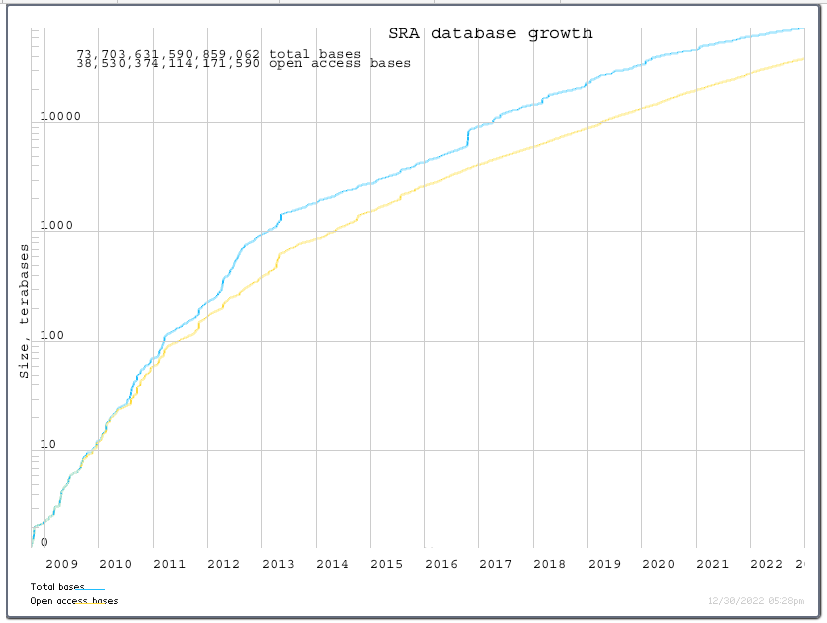
\includegraphics[width=0.95\textwidth]{images/SRA_data_growth.png}
% \caption{Sequence read archive (SRA) data growth. SRA data contains a trove of biological diversity information. Existing computational biology tools do not scale to support searching through all of SRA\@. This renders what is otherwise an immensely valuable public resource largely inert.}
% \label{fig:sra_data}
% \end{wrapfigure}


% GPUs have not seen widespread adoption in computational biology applications. For example, they are used in taxonomic classification of metagenomic data, indexing and searching through terabytes of raw sequencing data, constructing and querying pangenomic graphs.

%Anything that involves sophisticated data structures and when memory is constrained GPUs are not currently useful.

% GPUs are not currently used for many computational biology applications because efficient GPU data structures do not exist.
%\para{Requirements for building scalable dynamic and irregular GPU data structures}
%Data structures are the core of computational biology applications and are critical for their performance and scalability.
%To build scalable computational biology applications that can keep up with the rapid growth data we need compact, high-performance, dynamic, and distributed data structures. Specifically, we need: (1) approximate data structures such as filters, sketches, and locality-sensitive hashing data structures; and (2) exact data structures such as hash tables, string data structures, succinct data structures, and trees.
%
%These data structures and algorithms will need to exploit accelerators such as GPUs to scale up computations and at the same time support  features such as space-efficiency, dynamism, high concurrency, scaling out of GPU device RAM to host RAM, and distributed memory design to scale out to multiple nodes.
%%
%Furthermore, to achieve fine-grained resizing and to keep the peak memory usage low, we first need to develop new algorithmic approaches for traditional CPU data structures and then extend them to GPUs.
%}


\subsection{Computational Biology Applications and Associated Research Problems}
\label{subsec:target-applications}

\textbf{Metagenomic classification and abundance estimation} is the problem of assigning each read in a metagenomic sequencing sample to some likely taxon of origin.  This is a challenging task for many reasons, including the heterogeneity of the data (the sample being sequences can contains thousands of taxa and millions or more individual organisms), the incompleteness of the reference databases (the sample almost certainly contains species never before seen and absent from the database), and the complex sequence similarity relationships between the organisms in the sample (the organisms are related through a deep and often complex taxonomy).  The goal in this problem is to assign each read to the most specific taxon possible (e.g. if the read can't be associated with a species, assign a genus, etc.) or to leave the read as unclassified. The closely related problem of metagenomic abundance estimation asks to determine the distribution of abundances of taxa in a metagenomic sample, but does not require the specific allocation of individual reads, allowing e.g. the probabilistic or proportional allocation of individual sequencing reads.

Existing tools for metagenomic classification and abundance estimation~\cite{ames2013scalable, kim2016centrifuge, menzel2016fast, wood2014kraken, wood2019improved, dilthey2019strain,liu2018novel}, while popular and widely-used, suffer from memory bottlenecks (e.g. popular indexes can exceed 100~GB~\cite{simon2019benchmarking} especially when the reference data includes large eukaryotic genomes~\cite{meiser2017sequencing, knutson2017porcine}) and while designed to be fast, still struggle to keep pace with rapid new techniques of data acquisition.  An additional critical issue with most existing approaches is that, to reduce index sizes as much as possible, the indices they use are static and require full or near-full rebuilds whenever the reference databases upon which they rely are updated.

We plan to turn the algorithms and data structures we develop to the challenge of scalable metagenomic classification and abundance estimation. Our tool will rely on state of the art hashing and string indexing approaches to construct a succinct (updatable) reference index, and will take advantage of the massive parallelism available on the GPUs to dramatically speed up the tasks of taxonomic read assignment and statistical estimation of taxa abundance.

\begin{rproblem}%[\textbf{Metagenomic classification and abundance estimation at terabyte scale}]
Build a tool to perform reference-based taxonomic classification of metagenomic reads, and the associated taxonomic abundance estimation, for terabyte-scale metagenomic datasets. The software tool will support adding newly sequenced microbial genetic sequences to the database and updating the labels of existing ones without rebuilding the whole index.
\label{rprob:taxo-meta}
\end{rproblem}


\paragraph{Large-scale sequence search at SRA scale.} The BLAST~\cite{altschul1990basic} tool, which enables sequence-level search against the current database of assembled genomes, is one of the most widely-cited tools in science.  Yet, the vast majority of sequencing data has not been (and much of it will never be) assembled into a reference genome.  These raw data contain tremendous amounts of information about individual diversity, the relation of sequence level features to potential disease states, and novel (often functional) biological sequences that are not part of any reference genome.  Thus, enabling search over the raw collection of sequence data would be of tremendous utility to biological research.

The problem of searching for a query sequence against a vast collection of thousands or more raw sequence samples has recently been the focus of considerable research efforts.  The problem was first introduced by Solomon and Kingsford~\cite{solomon2016fast} and dubbed the experiment discovery problem. Those authors also proposed an algorithm and data structure, the Sequence Bloom Tree (SBT) that enables large-scale search (though still at orders of magnitude smaller scale that the large publicly available databases like the Sequence Read Archive~\cite{SRA} which remains the ultimate goal).

This challenge has subsequently been the focus of much work, including both approaches related to variations of the SBT data structure~\cite{SolomonK17,HarrisM20,BingmannBGI19}, and entirely distinct approaches proposed by PIs Pandey, Patro and Bender~\cite{PandeyAlBe18} and extended upon by PIs Pandey and Patro~\cite{AlmodaresiPFJP20} that relies on filters, hashing, and compressed inverted indexes.  There has also been promising recent work~\cite{Karasikov2020} relying on succinct string indexes like those we propose to enable on the GPU in this work.  Beyond simply representing the sequence content itself though, a key challenge among these approaches has been building a so-called ``color index'' that can efficiently map each indexed sequence back to its samples of origin. Highly-compressed representations exist~\cite{Karasikov2020,Pibiri2023MacDBG,AlmodaresiPFJP20}, but are (semi-)static. 

We propose to develop new algorithms, data structures, and software to help tackled the raw sequence search problem. Here, we will seek to leverage our work on building dynamic succinct data structure primitives to develop novel, compact, and \emph{updatable} sequence search representations, drawing on ideas from our prior work in compact static representations~\cite{AlmodaresiPFJP19,Pibiri2023MacDBG}.

\begin{rproblem}%[\textbf{Build a raw sequence search index at SRA scale}]
Build a search index over all (non-access-controlled) raw experiments present in SRA and enable interactive sequence-level searches. Host the search tool publicly to make it available for researchers around the world.
% Researchers can quickly ask biological questions and get answers.
% For example: what if researchers wants to determine: if a new putative disease-related transcript appeared in other samples, if a new fusion event is common among samples with a given subtype, which samples contain a new unexpected bacterial contaminant.
\label{rprob:seq-search}
\end{rproblem}

\noindent
\textbf{Pangenomics}~\cite{sherman2020pan} involves cataloging the genomes of individuals in a related population in the form of a sequence graph to preserve the variation across the individuals. This pangenome is used as the reference genome for the species and forms the basis of subsequent studies. Representing population variation (e.g. SNVs, indels, copy numbers, etc.) is critical to understanding relatedness, population diversity, and to avoiding reference bias during analysis and disease studies. These graphs represent a population-level reference, against which one can perform sequence-to-graph alignment. Even in the context of small and easy-to-sequence bacteria pan-genomes provided novel scientific insights and contributed to our understanding of underlying differences in pathogenicity, virulence and drug resistance~\cite{sherman2020pan}.

Cataloging the DNA from large populations of individuals in a species is a daunting task. Building a pangenome graph involves storing the genomic sequences of thousands or more individuals in the form of a sequence graph, where each path in the sequence graph follows the genome of an individual and has a unique coordinate system~\cite{pandey2021variantstore}. Query of and alignment to the graph must simultaneously weed out infeasible paths in the graph, and track the related but distinct coordinate systems of the different individuals indexed (given the absence of a single, uniform reference). Current approaches to this problem are computationally and memory intensive, despite substantial work to scale solutions up and out \cite{garrison2018variation,pandey2021variantstore}.

Simply put, current pangenomic indexes do not scale to population-scale variation datasets such as the 100,000 Genomes project~\cite{1002021100}, nor do 
existing pangenome indexes support easily adding new genomes to an existing index. In order to add a new genomic sample to the pangenomic requires index rebuilding. Finally, pangenomic indexes need to support fast variant queries and sequence-to-graph alignment. Achieving both of these operations in a single index is a challenging task. Existing tools are optimized for one of these operations but not both.

We seek to take advantage of the efficient dynamic succinct data structures, string indexing data structures, and scalable filtering data structures we will build in this proposal to develop algorithms capable of building a pangenomic index at population scale, performing sequence-to-graph alignment against this index, and performing fast variant queries against this index.

\begin{rproblem}%[\textbf{Building a pangenomic index at population-scale}]
 Build a pangenomic index that can perform fast variation queries and sequence-to-graph alignment at population-scale datasets available today. We further want to support adding new genomic samples to an existing index without rebuilding the index.
\label{rprob:pangenomics}
\end{rproblem}


\if 0
\subsection{Metagenome assembly}

% \begin{figure}
% \begin{wrapfigure}{R}{0.7\textwidth}
%     \centering
%     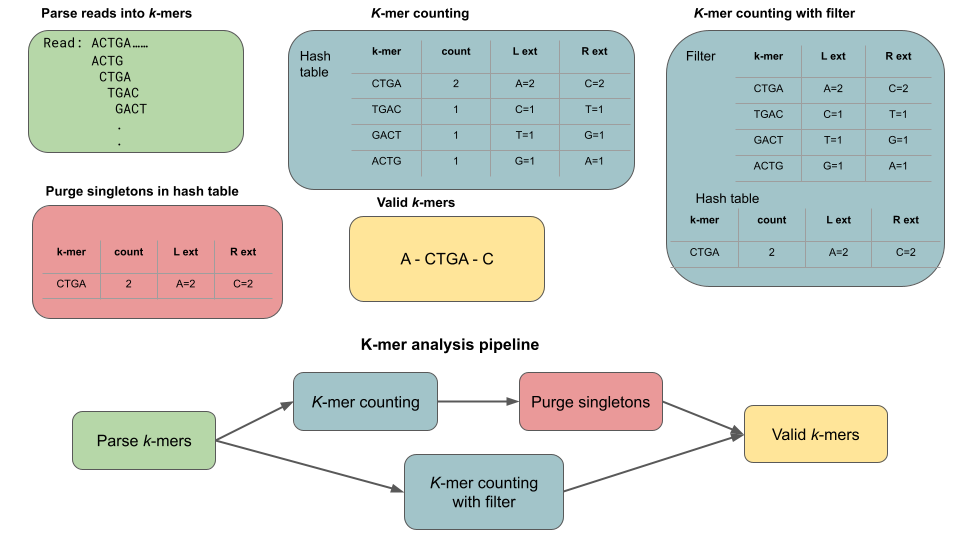
\includegraphics[width=0.9\linewidth]{images/mhm-pipeline.png}
%     \caption{The \textit{k}-mer analysis pipeline in MetaHipMer. A filter can help weed out singleton \kmers from being inserted into the hash table.}
%     \vspace{-0.5em}
%     \label{fig:mhm-kmer}
% \end{wrapfigure}
% \end{figure}

\textbf{Problem definition.}
Metagenome assembly involves reconstructing long contiguous sequences (\emph{contigs}) of genetic material from short input \emph{reads}~\cite{yang2021review}. These reads are strings of bases (the DNA alphabet A, C, G, T) of length 150 to 250 that are produced by gene sequencing machines.
For metagenomes, these reads are extracted from environmental samples (e.g., gut bacteria, or a soil sample) that contain the genes of potentially thousands of microbes, existing at varying abundances.
The reads are error-prone (typically about 0.24\% error per base) and sequencing is done multiple times to ensure every region of genetic material is covered with some error free sequences.

\noindent
\textbf{Importance.}
Metagenomic sequencing provides a culture-independent avenue to investigate the complex microbial communities by constructing metagenome-assembled genomes (MAGs). A MAG represents a microbial genome by a group of sequences from genome assembly with similar characteristics. It enables us to identify novel species and understand their potential functions in a dynamic ecosystem.

\begin{wraptable}{r}{4.5in}
\centering
%\resizebox{\columnwidth}{!}{%
    \begin{tabular}{c c c c c c}
    \toprule
    \textbf{Dataset} & \multicolumn{5}{c}{\textbf{Percentage singleton \kmers}} \\
    \midrule
    & $k=21$ & $k=33$ & $k=55$ & $k=77$ & $k=99$ \\
    \midrule
    WA &  66 & 73 & 76 & 78 & 78  \\
    Rhizo &  67 & 75 & 80 & 83 & 85  \\
    Tymeflies & 63 & 62 & 67 & 69 & 71 \\
    \bottomrule
    \end{tabular}
 %   }
    \caption{Distribution of singleton \kmers in metagenomic data for values of $k$.}
    \label{tab:kmer-dist}
\end{wraptable}

\noindent
\textbf{Challenges.}
Metagenome assembly is challenging due to sequencing error, repetitive content, and library and sequencing bias. In addition, a metagenome sample can contain many thousands of different genomes with varying degrees of similarity, sometimes sharing genetic material, and occurring at vastly different abundances.
%
Furthermore, high-throughput sequencing technology is producing large-amount of metagenomic datasets ranging to TB and PB scales~\cite{hofmeyr2020terabase}. Metagenomic assembly is a complex process consisting of multiple phases and scaling all these phases to terabyte scale comes with a myriad of challenges.

\noindent
\textbf{State of the art.}
MetaHipMer~\cite{GeorganasEHG18,hofmeyr2020terabase} is the first exascale metagenome assembler.
In the approach used by MetaHipMer, the reads are first divided into overlapping substrings of fixed length \emph{k}, called \emph{\kmers}, which are then used to form a de Bruijn graph~\cite{CompeauPeTe11}.
\Kmer counting is the very first step. During \kmer counting, forward and backward extensions of the \kmer and the counts of those extensions are also maintained in the hash table along with the \kmer. Information regarding the extensions and their counts is critical to identifying correct paths in the de Bruijn graph and requires 28 to 52 bytes (depending on $k$) to store each \kmer.
MetaHipmer uses GPUs to speed up the \kmer analysis phase.
In a de Bruijn graph, the vertices are \kmers and edges connect any two \kmers that have an overlap of $k-1$ bases. These vertices are stored in a hash table that is distributed across all the compute nodes in a supercomputer like Perlmutter~\cite{perlmutter} or Summit~\cite{summit}.
Traversal of the de Bruijn graph enables the construction of the contigs (longer sequences).  This approach is more efficient than an all-to-all alignment of the reads, which would be prohibitive for the size of typical metagenome datasets (up to billions of reads).

\noindent
\textbf{Gap and requirements.}
\Kmer counting and analysis is the very first and the most memory-intensive step in the metagenome assembly. The \kmers that occur only once (singletons) are treated as sequencing errors and dropped. In a typical set of metagenome reads, 70--80\% of unique \kmers are singletons, but they still need to be stored and counted in the distributed hash table (see~\Cref{tab:kmer-dist}).
In the default MetaHipMer implementation, storing the unique \kmers is the most memory-intensive part of the computation and can be roughly an order of magnitude larger than the input data.  The space required to store the \kmers can be much larger than the size of the original raw dataset (up to $10\times$ larger) as \kmers contain a lot of redundant information due to their overlaps.
Weeding out singleton \kmers before inserting them in the hash table to count is critical in any \kmer analysis phase to reduce the memory usage of the counting phase. These singleton \kmers can also be pruned from the hash table after the counting phase. However, that results in the high peak memory usage and much slower running time. MetaHipMer uses filers to weed out singleton \kmers.

The size of the filter and hash table is dependent on the number of unique \kmers. Given that the distribution of \kmers is highly skewed and not known in advance, it is challenging to size the filter and the hash table in order to efficiently utilize the limited memory. Filter and hash tables that can be efficiently resized at runtime will enable efficient memory utilization.


\begin{rproblem}[\textbf{Scale MetaHipMer to petabyte-scale metagenomic datasets on supercomputers}]
Accelerate \kmer analysis phase in MetaHipMer using GPUs and reduce the peak RAM usage to support assembly of petabyte-scale metagenomic datasets from complex biological environments.
\label{rprob:metahipmer}
\end{rproblem}

\fi